%%%%%%%%%%%%%%%%%%%%%%%%%%%%%%%%%%%%%%%%%
% a0poster Portrait Poster
% LaTeX Template
% Version 1.0 (22/06/13)
%
% The a0poster class was created by:
% Gerlinde Kettl and Matthias Weiser (tex@kettl.de)
% 
% This template has been downloaded from:
% http://www.LaTeXTemplates.com
%
% License:
% CC BY-NC-SA 3.0 (http://creativecommons.org/licenses/by-nc-sa/3.0/)
%
%%%%%%%%%%%%%%%%%%%%%%%%%%%%%%%%%%%%%%%%%

%----------------------------------------------------------------------------------------
%	PACKAGES AND OTHER DOCUMENT CONFIGURATIONS
%----------------------------------------------------------------------------------------

\documentclass[a0,portrait]{a0poster}

\usepackage{multicol} % This is so we can have multiple columns of text side-by-side
\columnsep=50pt % This is the amount of white space between the columns in the poster
\columnseprule=0pt % This is the thickness of the black line between the columns in the poster




\usepackage[svgnames]{xcolor} % Specify colors by their 'svgnames', for a full list of all colors available see here: http://www.latextemplates.com/svgnames-colors

\usepackage{qrcode}

%\usepackage{times} % Use the times font
%\usepackage{palatino} % Uncomment to use the Palatino font
\usepackage[sfdefault]{FiraSans}

\usepackage{graphicx} % Required for including images
\graphicspath{{figures/}} % Location of the graphics files
\usepackage{booktabs} % Top and bottom rules for table
\usepackage[font=small,labelfont=bf]{caption} % Required for specifying captions to tables and figures
\usepackage{amsfonts, amsmath, amsthm, amssymb} % For math fonts, symbols and environments
\usepackage{wrapfig} % Allows wrapping text around tables and figures
\usepackage{microtype}

\definecolor{faimsorange}{HTML}{f28d09}
\definecolor{faimsblue}{HTML}{223884}
% https://tex.stackexchange.com/a/583319

\AddToHook{shipout/background}{%
    %\put (0in,-\paperheight){
\includegraphics[width=\paperwidth]{figures/faims3-orange-slide-background.png}}%
    \put (1in,-0.148\paperheight){
\includegraphics[width=\paperwidth]{figures/a0-blueback-faims.png}}%
    %\put (1in,-1213mm){
\includegraphics[width=\paperwidth]{figures/a0-faimsorange-footer.png}}%
}


\usepackage{sectsty}

\sectionfont{\color{faimsorange}}  % sets colour of sections
\subsectionfont{\color{black}}  % sets colour of sections
\usepackage[skip=10pt plus1pt, indent=0pt]{parskip}

\usepackage{caption}
\usepackage{subcaption}

\begin{document}

%----------------------------------------------------------------------------------------
%	POSTER HEADER 
%----------------------------------------------------------------------------------------

% The header is divided into two boxes:
% The first is 75% wide and houses the title, subtitle, names, university/organization and contact information
% The second is 25% wide and houses a logo for your university/organization or a photo of you
% The widths of these boxes can be easily edited to accommodate your content as you see fit

\begin{minipage}[b]{0.75\linewidth}
\veryHuge \color{White} \textbf{FAIMS 3.0 Electronic Field Notebooks} \color{faimsorange}\\[0.5cm] % Title
\Huge\textit{Project Update}\\[2cm] % Subtitle
\large \color{white} \textbf{Penny Crook\textsuperscript{1}}, Shawn Ross\textsuperscript{1}, Brian Ballsun-Stanton\textsuperscript{1}, Steve Cassidy\textsuperscript{1}, \textbf{Jens Klump\textsuperscript{2}}, \& Adela Sobotkova\textsuperscript{3}\\[0.5cm] % Author(s)
\end{minipage}
%
% \begin{minipage}[b]{0.25\linewidth}
% \hspace{.15\linewidth}
% 
\includegraphics[width=15cm]{figures/FAIMS-Logo.pdf}\\
% \end{minipage}

%\vspace{1cm} % A bit of extra whitespace between the header and poster content

%----------------------------------------------------------------------------------------
\vfill

\begin{multicols}{3} % This is how many columns your poster will be broken into, a portrait poster is generally split into 2 columns

%----------------------------------------------------------------------------------------
%	ABSTRACT
%----------------------------------------------------------------------------------------
\begingroup
{
\color{faimsblue} % Navy color for the abstract


The Field Acquired Information Management Systems (FAIMS) Project has been supporting researchers in offline digital data capture and management on Android devices since 2014. In 2020 the Australian Research Data Commons (ARDC) and 19 partners invested in us to rebuild the FAIMS Mobile Platform from the ground up. Our new software, FAIMS3, is cross-platform (Android, iOS and desktop), offers more flexible synchronisation, new integrations, a DIY option for customisation, and a sleek new look. As we prepare for its public release in 2023 we present the current set of features, those on the roadmap for future development, and our plans for sustaining this open-source software in a commercial setting.}
\endgroup
\color{Black} % Navy color for the abstract

%----------------------------------------------------------------------------------------
%	INTRODUCTION
%----------------------------------------------------------------------------------------

%\color{SaddleBrown} % SaddleBrown color for the introduction

\section*{Introduction}

The \textbf{FAIMS Mobile Platform} is open-source software for offline data collection. FAIMS stands for \textbf{Field Acquired Information Management Systems}. The platform was established by archaeologists at UNSW Sydney in \textbf{2012}. It is now based at Macquarie University and used by researchers from many fields in diverse situations. In 2020 the Australian Research Data Commons (ARDC) and 19 partners invested in us to rebuild the FAIMS Mobile Platform from the ground up (ARDC Platforms project doi: 10.47486/PL110). 

In partnership with the Australian Research Data Commons (ARDC) and 19 research and institutional partners, the \textbf{FAIMS 3.0 Project} has been rebuilding the FAIMS Mobile app from the ground up. We are working with developers at Australian Astronomical Optics Macquarie (AAO) to customise our software stack to enable cross-platform data collection (Android, iOS and desktop), more flexible synchronisation, integration with other platforms, a DIY option for customisation, and a sleek new look.

The open-source tool will be released in \textbf{April 2023} under a new name: \textbf{Fieldmark}. From July \textbf{Electronic Field Notebooks Pty Ltd} will commence offering hosting services for Fieldmark.

%\vspace{1cm}

%----------------------------------------------------------------------------------------
%	OBJECTIVES
%----------------------------------------------------------------------------------------

%\color{DarkSlateGray} % DarkSlateGray color for the rest of the content



\section*{Application Design}

FAIMS 3.0 allows teams to create \textbf{custom} mobile applications for \textbf{offline} field data collection--on consumer-grade hardware--without having to write or maintain code.

We use \textbf{React}, \textbf{Capacitor}, and \textbf{PouchDB} to collect, edit and export data--structured, geospatial, instrument, and multimedia data--on Android, iOS, and the web. 



\subsection*{Workflow}
A FAIMS3 data-collection project \textbf{starts with a workflow}, preferably an established one. It may begin in a paper form and companion manual, a well-crafted digital package or an export from a prior project.


The field director (or delegated person) then makes the \textbf{notebook specification} on our (online) \textbf{notebook creator} to suit the data needed. (We don’t support multi-person notebook editing at present, so one and only one person should be responsible for the notebook design.) 

We then \textbf{deploy the notebook on appropriate servers}. The team can deploy FAIMS3 onto several devices through various channels: \textbf{Android}, \textbf{web}, and \textbf{iOS}. As they are deploying devices, the team should also be registering and communicating their usernames (currently through FAIMS3 administrators). (Project leads will eventually manage the deployment of notebooks and management of users themselves.)


Once \textbf{synchronised, data collection can begin.} Users can bring tablets and phones and laptops out into the field to collect data. (Specifically, we support record creation, retrieval, updating, and deletion.) We have demonstrated using external Bluetooth GPS receivers and support onboard camera and external file attachments for photos and multimedia. 

%Thus, we have a team, while offline, collecting geospatial and multimedia data in addition to structured data as specified in their workflow.

% \endgroup

 


\textbf{Then, once back from fieldwork, data can be exported.} This export can utilise a variety of formats and APIs.

\columnbreak
\begin{center}
 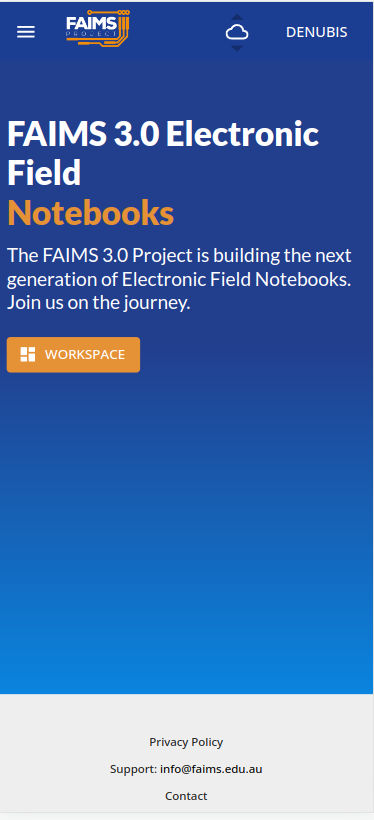
\includegraphics[width=.32\columnwidth]{figures/Screenshot from 2022-10-13 10-54-38.png}
 \hfill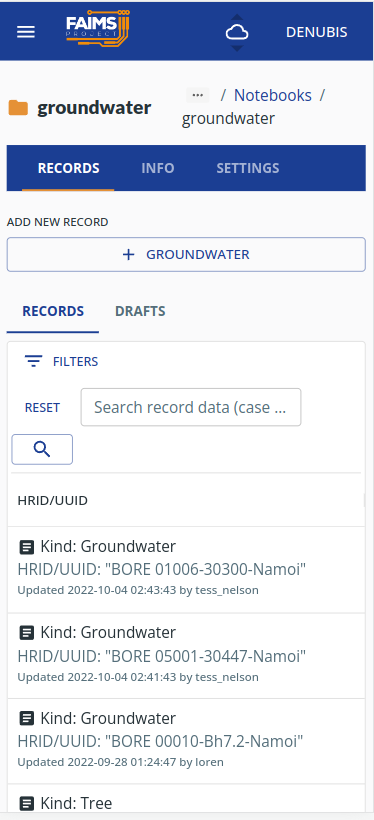
\includegraphics[width=.32\columnwidth]{figures/Screenshot from 2022-10-13 10-54-28.png}
 \hfill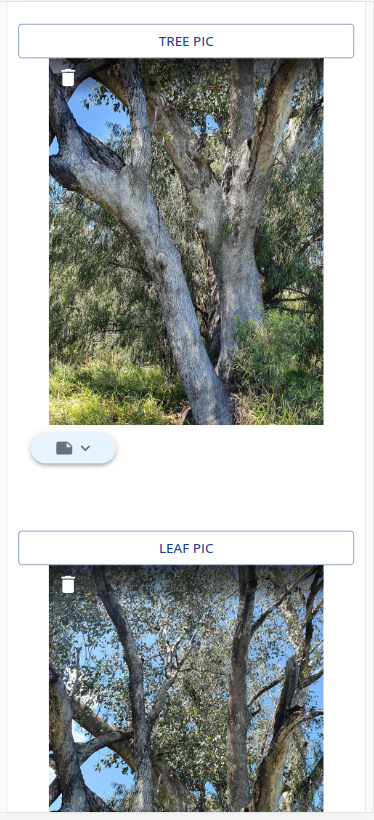
\includegraphics[width=.32\columnwidth]{figures/Screenshot from 2022-10-13 10-56-01.png}
\captionof{figure}{FAIMS3 beta screenshots with data from recent Macquarie University Faculty of Science and Engineering fieldwork collecting groundwater and vegetation data in NSW.}

\end{center}


\subsection*{Architecture}
\begin{center}

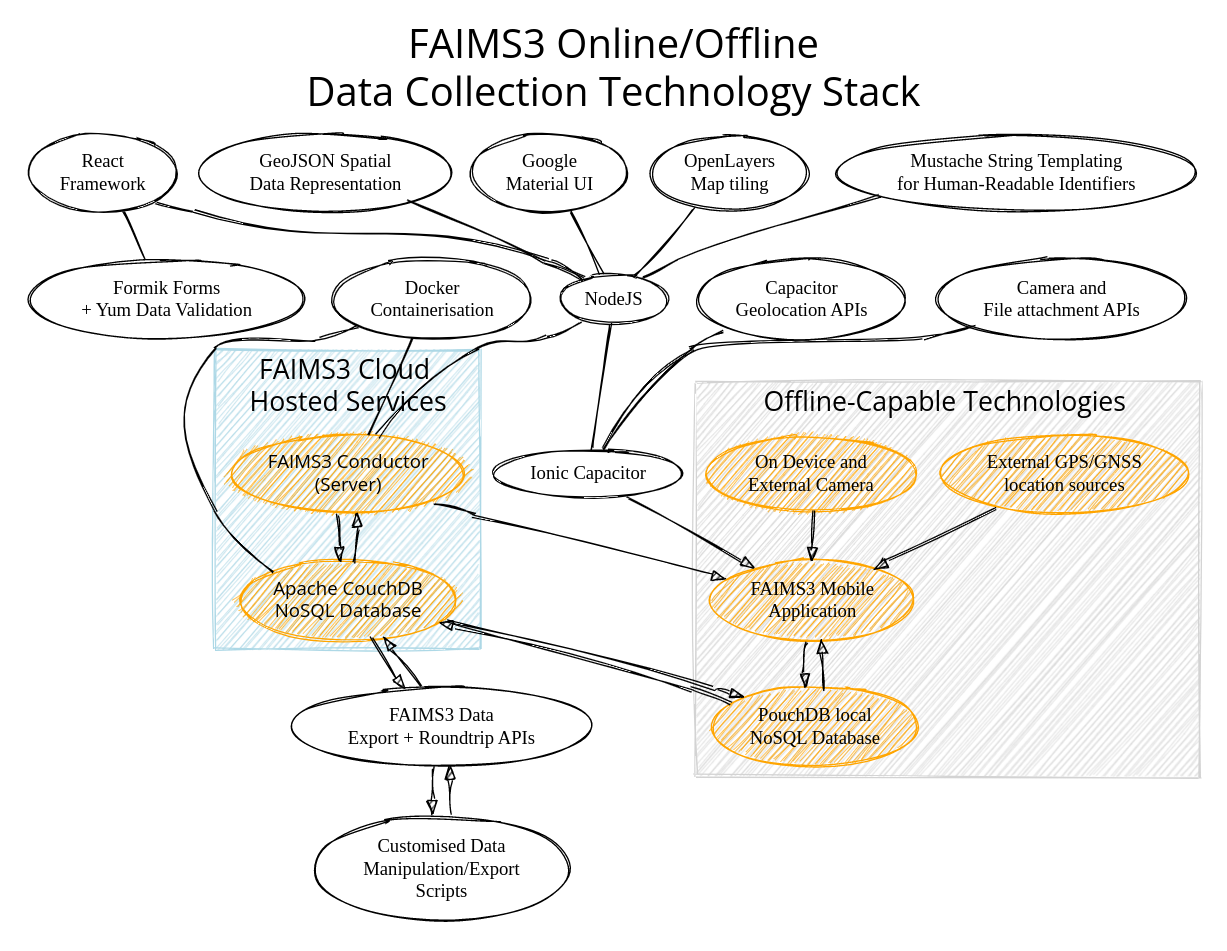
\includegraphics[width=\linewidth]{figures/faims3-tech-diagram.png}
\captionof{figure}{FAIMS3 Data flow and schematic architecture.}
\end{center}


The FAIMS3 web-app: the app, itself, is written in Javascript (\textbf{NodeJS ← React ← Formik ← Yum, Material UI, OpenLayers, Capacitor, Moustache}). When presented on the browser, the browser receives a static site (HTML + compiled/minified JS + CSS + binary assets). The app uses PouchDB as a local, offline-capable, NoSQL datastore. It reaches out to our server to generate a JWT authentication token.

Our lightweight server, \textbf{the Conductor}, handles role management and authentication. It however, does not perform data exchange. The Conductor mints tokens, will eventually be able to moderate, edit, and create notebook designs, and will handle being a wrapper for our CouchDB datastore for other clients and non-FAIMS3 users.

\textbf{PouchDB} uses the JWT token to replicate with a central \textbf{Apache CouchDB} datastore running in a Docker container. The reason we chose CouchDB/PouchDB was because full replication (copy and sync) running in an `eventual synchronisation' state (i.e. when the database can see the network again) was very exciting to us. We did not have to write an offline-capable data synchronisation protocol.

Once all notebook metadata and data are synchronised, a properly authenticated user can load visible notebooks and visible records. Once this initial sync is performed the app is entirely equipped for offline fieldwork.

\textbf{The FAIMS3 mobile app} is all of the above, except instead of NodeJS, Ionic’s CapacitorJS transpiles the javascript + extra components and plugins into native code for iOS and Android. Pragmatically, it is the same technology used by Electron to wrap a web browser and an extremely specific set of pages in an executable wrapper. As a hybrid native app, however, we can access the device-specific APIs for geolocation, camera, and Bluetooth — functionality critical for arbitrary workflows. Capacitor offers many plugins in this vein.



\columnbreak

\textbf{Roundtrip and Export} scripts are presently written in Python and connect directly to the CouchDB servers. By using our own library, we can translate the form → record → revision → attribute-value-pair NoSQL appropriate format of our internal datastore into dataframes appropriate for manipulation and export. These scripts can create new revisions (changing field values and record metadata like deleted flags) as well as exporting single entries or an entire workflow's datastore. Once in a more computable format, scripts then rename photos and files, organise everything, and export to csv, xlsx, KML, and GeoJSON.





% \endgroup



\section*{Sustainability}
% \begingroup
% \setlength{\columnsep}{25pt}%
% \begin{wrapfigure}{r}{0.2\textwidth}
    
%\begin{center}
% 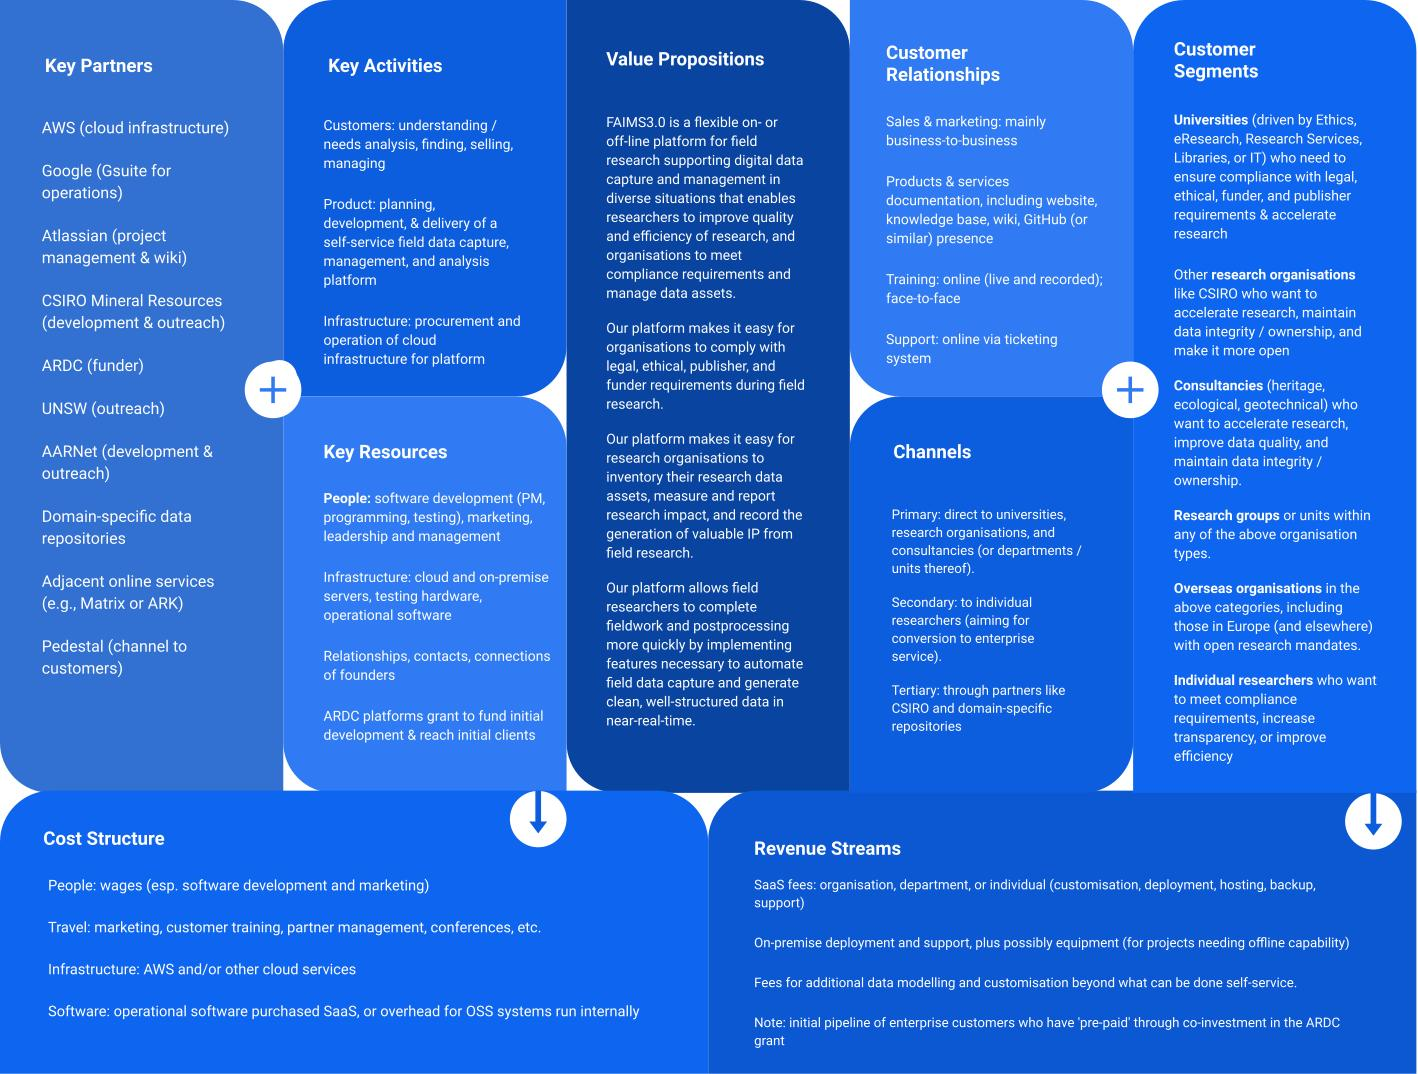
\includegraphics[width=0.35\textwidth]{01-FAIMS3-business-canvas.jpg}
% \caption{\color{Green} Electronic Field Notebook Pty Ltd Business Canvas}
%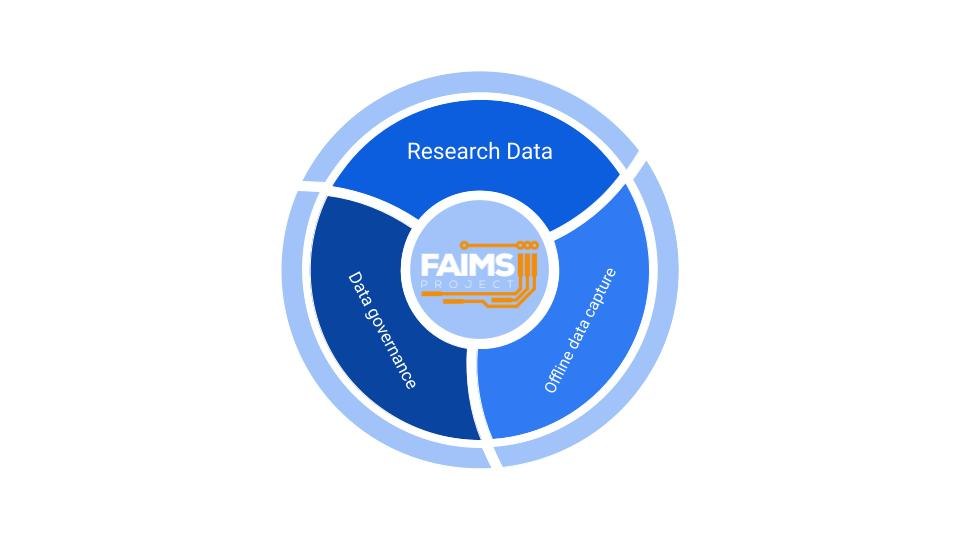
\includegraphics[width=0.2\textwidth]{FAIMS-target.jpg}
%\captionof{figure}{Focus of FAIMS3 software design: offline, compliant research data.}
%\end{center}
% \end{wrapfigure}

The FAIMS Project has a 10-year record of successful software development, deployment, client support and community-building. 

Drawing on our experience with the CSIRO ON Prime Program (2016), including 70+ interviews with users and potential adopters, we carefully refined our technological priorities to meet user needs. The new system will be self-service, cross-platform and retain the core features of the old software with enhanced performance. 

\subsection*{Commercialisation}

With an open-source core supporting research transparency but value-adding services that can generate revenue to share the cost of long-term maintenance of the software. This is the COSS model.

We have established a company, Electronic Field Notebooks Pty Ltd, which is currently based at the Macquarie Incubator. This program has energised and accelerated our commercialisation plans as we revisit value propositions, customer segments and refine our pitch.

It is clear that in a marketplace of open-source and proprietary tools for research data collection and offline data collection, the specialised needs of researchers collecting field data--of their own design--in offline settings in a fashion that enables FAIR-sharing of their data, compliant with the needs of their institution and funding bodies remains unmet. 
\vspace{1cm}
\begin{center}
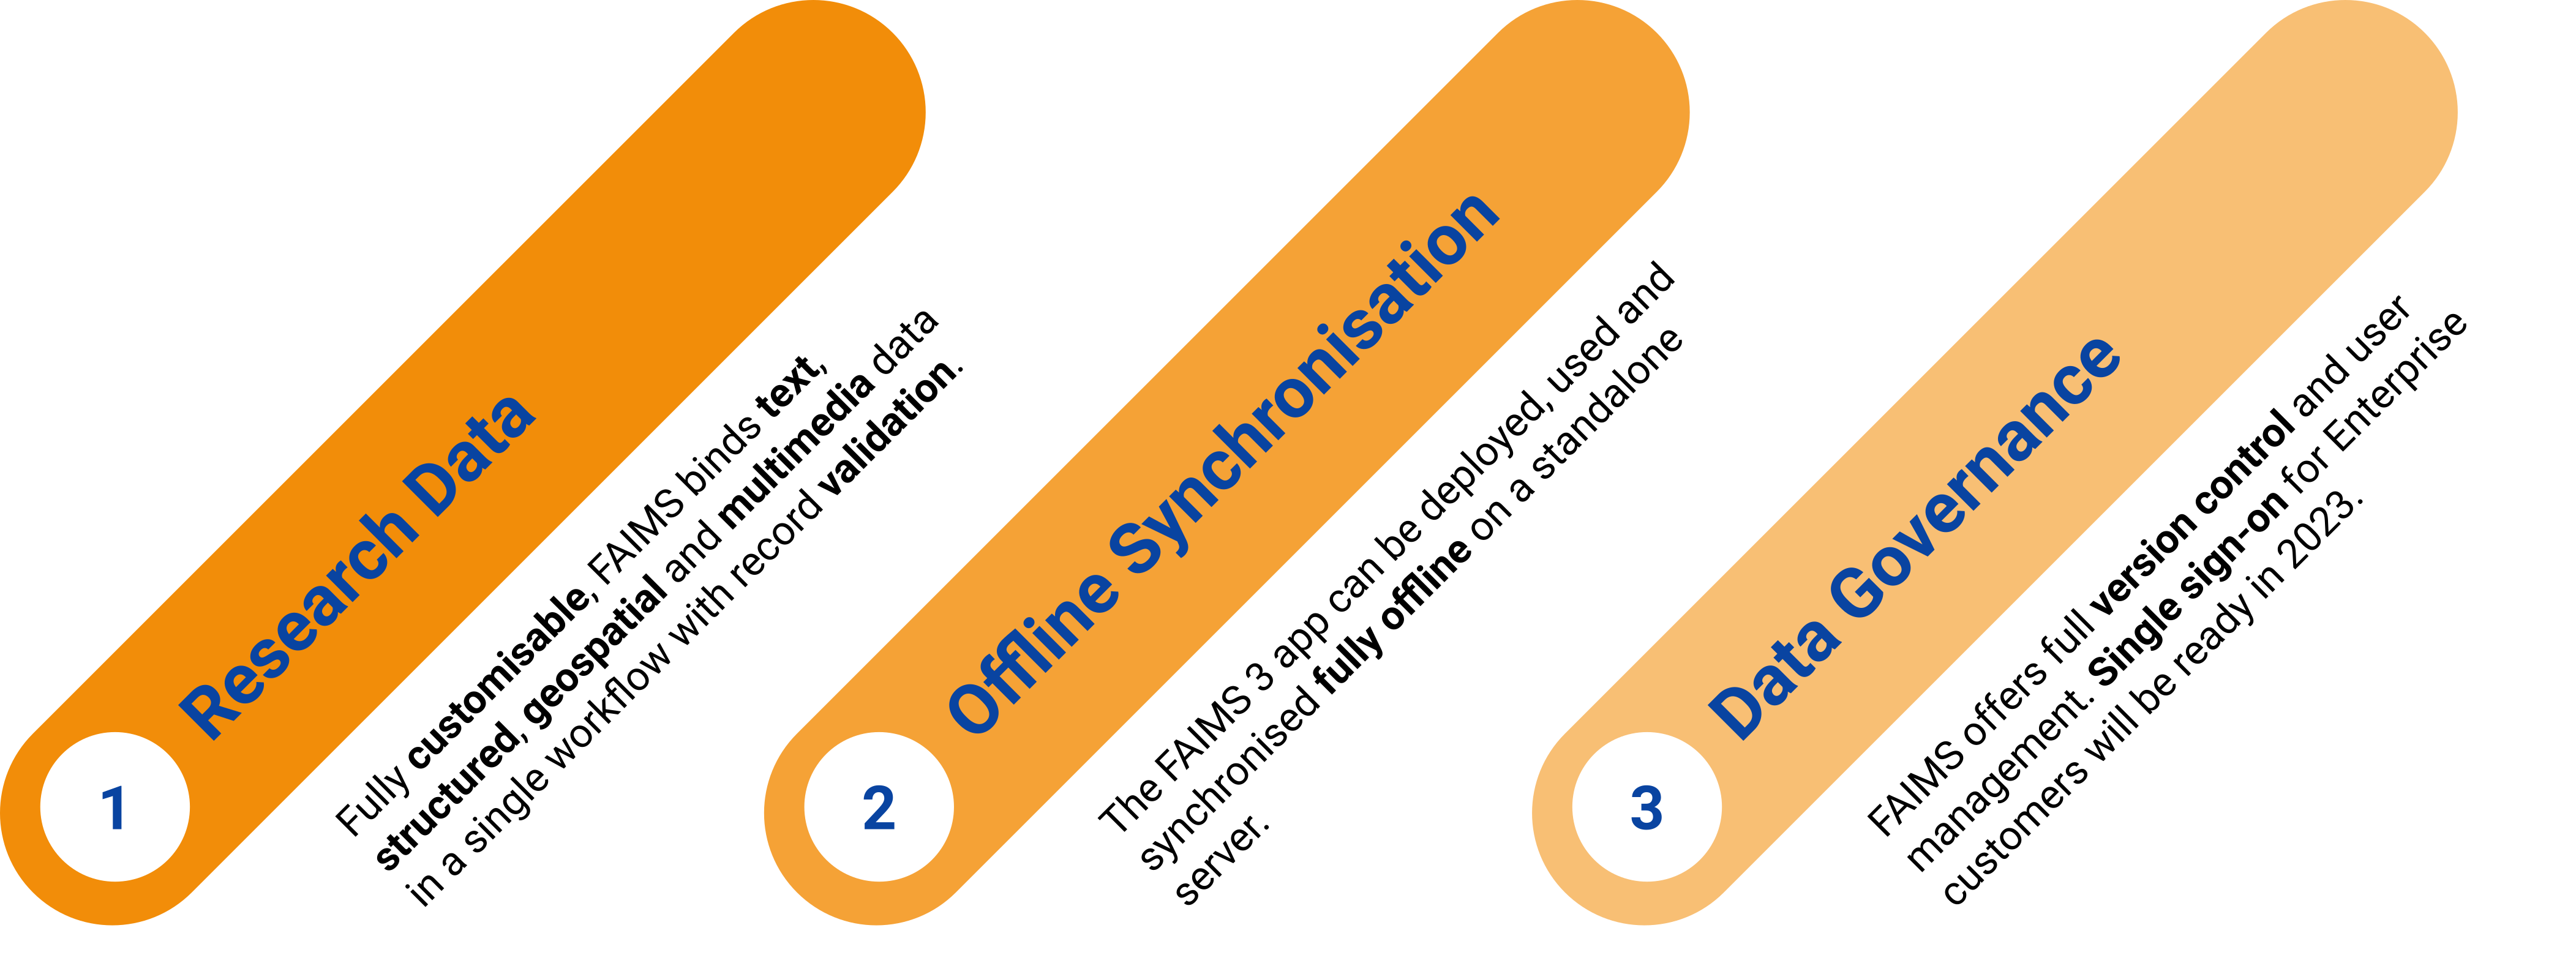
\includegraphics[width=\linewidth]{figures/marketing-materials.png}

\captionof{figure}{Focus of FAIMS3 software design: flexible, offline and compliant research data.}
% 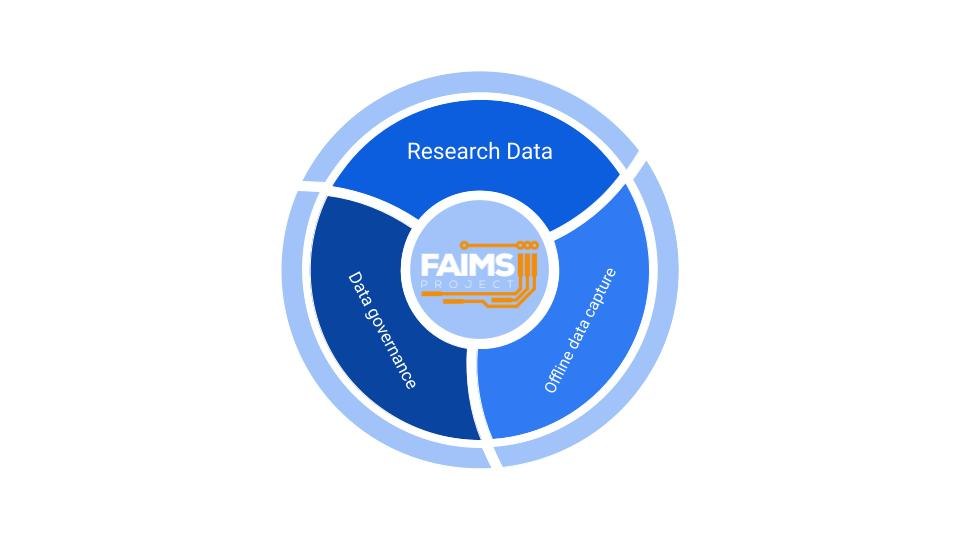
\includegraphics[width=0.2\textwidth]{FAIMS-target.jpg}
% \captionof{figure}{\color{Green} Focus of FAIMS3 software design: offline, compliant research data.}
\end{center}

\section*{Early adopters}

Our current beta software has been deployed by research and commercial teams for pilot projects at Macquarie University, CSIRO and Aarhus University. We are learning much about the limitations and possibilities of our new architecture.


\begin{center}
    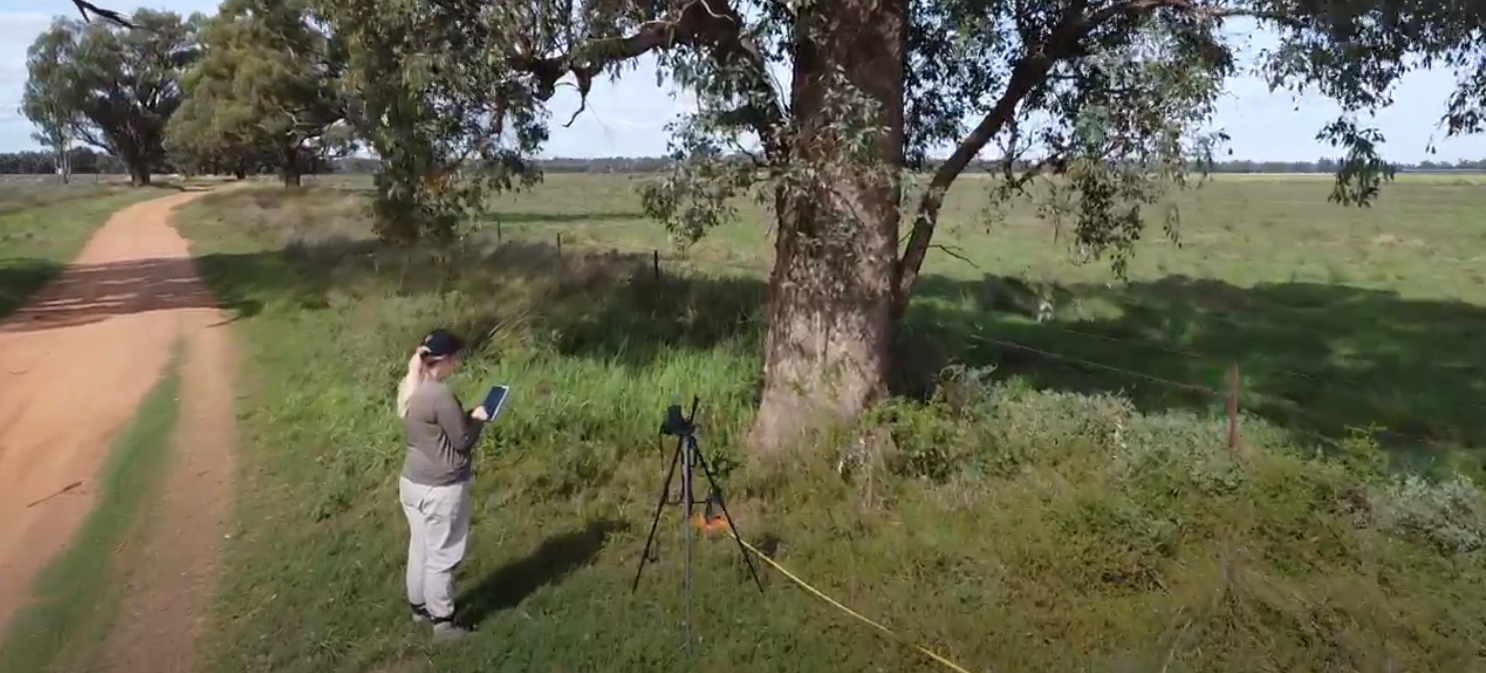
\includegraphics[width=\linewidth]{figures/Screenshot from 2022-10-13 10-58-35.png}
    \captionof{figure}{Macquarie University Faculty of Science and Engineering researchers collecting near-bore vegetation data.}
\end{center}



% \subsection*{Timeline}

% \begin{enumerate}

% \item[2012 ] FAIMS Project launched at University of New South Wales with NeCTAR eResearch Tools grant 

% \item[2014 ] FAIMS 1.0 released \textbf{+} FAIMS Project awarded and ARC Linkage Infrastructure Equipment and Facilities grant

% \item[2015 ] The FAIMS Project moved to Macquarie University \textbf{+} FAIMS 2.0 released

% \item[2016 ] The FAIMS Project begins operating as open-source software consultancy \textbf{+} Awarded NSW RAAP grant from NSW government (2016 to 2018) \textbf{+} FAIMS undertakes market analysis via CSIRO ON Prime

% \item[2017 ] FAIMS 2.5 released

% \item[2018 ] FAIMS wins US Bureau of Reclamation / US Geological Survey innocentive.com prize for ‘FAIMS 3.0’ proposed design

% \item[2019 ] Successful ARDC Platforms investment

% \item[2020 ] Commenced 'FAIMS 3.0 Electronic Field Notebooks' Project

% \item[2021 ] Alpha v0.1.0 was released (internally) in June \textbf{+} Beta v0.3.0 was released (internally) in December

% \item[2022 ] Production version will be available for limited release in \textbf{December}.

% \item[2023 ] Public release of open-source tool \textbf{Fieldmark} in \textbf{April} \textbf{+} Electronic Field Notebooks Pty Ltd will commence offering hosting services for Fieldmark in \textbf{July}. 
% \end{enumerate}




% \endgroup

% \begin{center}\vspace{1cm}
% 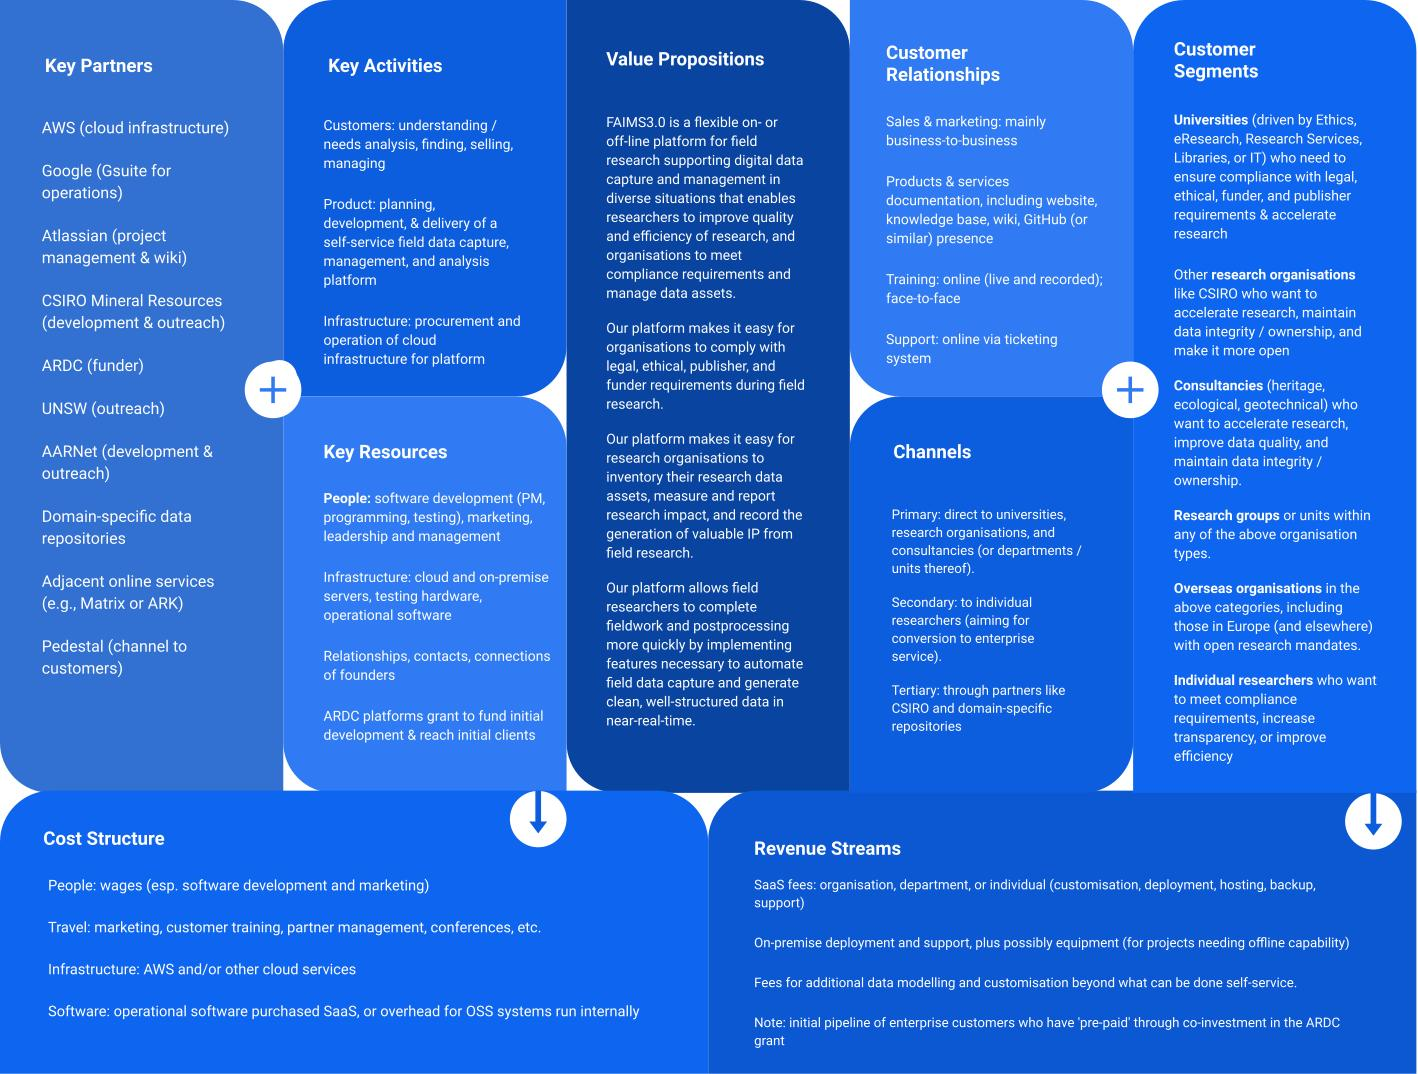
\includegraphics[width=0.9\linewidth]{01-FAIMS3-business-canvas.jpg}
% \captionof{figure}{\color{Green} Electronic File Notebook Pty Ltd Business Canvas}
% \end{center}\vspace{1cm}

%----------------------------------------------------------------------------------------
%	CONCLUSIONS
%----------------------------------------------------------------------------------------

% % \vspace{2cm}
% \color{SaddleBrown} % SaddleBrown color for the conclusions to make them stand out

% \section*{Conclusions}

% \begin{itemize}
% \item Pellentesque eget orci eros. Fusce ultricies, tellus et pellentesque fringilla, ante massa luctus libero, quis tristique purus urna nec nibh. Phasellus fermentum rutrum elementum. Nam quis justo lectus.
% \item Vestibulum sem ante, hendrerit a gravida ac, blandit quis magna.
% \item Donec sem metus, facilisis at condimentum eget, vehicula ut massa. Morbi consequat, diam sed convallis tincidunt, arcu nunc.
% \item Nunc at convallis urna. isus ante. Pellentesque condimentum dui. Etiam sagittis purus non tellus tempor volutpat. Donec et dui non massa tristique adipiscing.
% \end{itemize}

% \color{DarkSlateGray} % Set the color back to DarkSlateGray for the rest of the content

%----------------------------------------------------------------------------------------
%	FORTHCOMING RESEARCH
%----------------------------------------------------------------------------------------

% \section*{Forthcoming Research}

% We have a newsletter at \texttt{faims.substack.com}.

%----------------------------------------------------------------------------------------
%	ACKNOWLEDGEMENTS
%----------------------------------------------------------------------------------------
\end{multicols}
\vfill
\hspace{-6cm}
\includegraphics[width=1.1\paperwidth]{figures/a0-faimsorange-footer.png}
\begin{multicols}{3}




\textsuperscript{1}Macquarie University; \textsuperscript{2}Exploration Through Cover, CSIRO; \textsuperscript{3}Aarhus University 

\vfill

This poster has been prepared for the eResearch Australasia Conference, Brisbane, 17–20 October 2022, using \LaTeX{}.

\vfill

This poster's PDF and code is available at: https://osf.io/5karu/

\vfill

\textbf{License:} This poster is CC-BY-SA. FAIMS3 uses Apache2. 




\section*{Contact}
\begingroup
\setlength{\columnsep}{25pt}
\begin{wrapfigure}{r}{.225\linewidth}
\centering
\vspace{3.5mm}
\qrcode[hyperlink,height=\linewidth]{https://faims.edu.au}
\end{wrapfigure}


\textbf{Dr Penny Crook}, Co-Director FAIMS Project, Macquarie University, penny@faims.edu.au

\textbf{Dr Jens Klump}, Group Leader Exploration Through Cover, CSIRO, jens@faims.edu.au

For more information visit \textbf{faims.edu.au}
\endgroup

\columnbreak

\section*{Acknowledgements}

\begin{center}


\includegraphics[width=\linewidth]{figures/FAIMS-keypartners.png}
%\captionof{figure}{FAIMS3 Data flow and schematic architecture.}
\end{center}

\end{multicols}
%----------------------------------------------------------------------------------------


\end{document}